\documentclass[convert={density=900,size=1080x800,outext=.png}]{standalone}
\usepackage{tikz}

\usetikzlibrary{calc, positioning}
\usetikzlibrary{arrows.meta}
\usetikzlibrary{matrix}
\usetikzlibrary{shadows}
\usepgflibrary{shapes.misc}
\usepgflibrary{{shapes.geometric}}

\pgfdeclarelayer{shadow} 
\pgfsetlayers{shadow,main}
\def\shadowradius{3pt}


\def\mw{2cm}
\def\mh{1.75cm}
\def\trianglecoordinate{2mm}

\newcommand\drawshadowbis[1]{
    \begin{pgfonlayer}{shadow}
        \fill[inner color=black,outer color=white] ($(#1.south west)$) circle (\shadowradius);
        \fill[inner color=black ,outer color=white] ($(#1.north west)$) circle (\shadowradius);
        \fill[inner color=black ,outer color=white] ($(#1.south east)$) circle (\shadowradius);
        \fill[inner color=black,outer color=white] ($(#1.north east)$) circle (\shadowradius);
        \fill[ top color=black, bottom color=white] ($(#1.south west)+((0,-\shadowradius)$) rectangle ($(#1.south east)$);
        \fill[left color=black,right color=white] ($(#1.south east)$) rectangle ($(#1.north east)+((\shadowradius,0)$);
        \fill[bottom color=black,top color=white] ($(#1.north west)$) rectangle ($(#1.north east)+((0,\shadowradius)$);
        \fill[right color=black,left color=white] ($(#1.south west)$) rectangle ($(#1.north west)+(-\shadowradius,0)$);
    \end{pgfonlayer}
    }

\tikzstyle{component} = [draw, fill=white, minimum width=\mw, minimum height=\mh, align=center]

\tikzset{
    border/.style = { 
        draw, rectangle, minimum width=\mw, minimum height=\mh, thick, align=center, ultra thick
    },
    Component/.pic = {
        \node [border](-edge){#1}; 
        \draw[thick] ([xshift=\trianglecoordinate] -edge.south) -- ([yshift=\trianglecoordinate] -edge.south);
        \draw[thick] ([xshift=-\trianglecoordinate] -edge.south) -- ([yshift=\trianglecoordinate] -edge.south);
        \draw[thick] (-edge.south) |- ++(-3mm, -4mm) node[xshift=-2mm, yshift=-1mm] {T}; 
    },
}

\tikzset{
    clockborder/.style = { 
        trapezium, trapezium angle=60, minimum width=1cm, draw, very thick
    },
    Clock/.pic = {
        \node [clockborder, shape border rotate=-180](-clockedge){#1};
        \draw[very thick] (-clockedge.east) -- ++(2cm, 0cm);
        \def\sft{0.5}
        \foreach \x in {0, 0.5, 1, 1.5}{
            \draw[very thick] (\x + \sft, 0.1) -| ++(0.25cm, 0.25cm) -| ++ (0.25cm, -0.25cm);
        }
    },
}

\begin{document}
    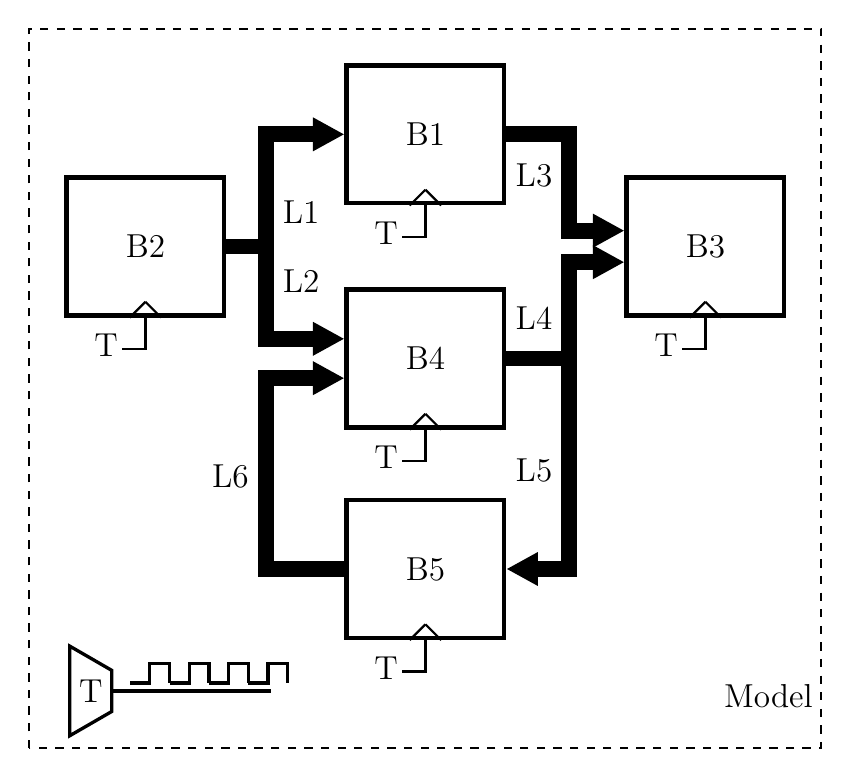
\begin{tikzpicture}[every node/.style={font=\large}]
        % Place the blocks 
        \matrix (m) [matrix of nodes, ampersand replacement=\&, column sep = 1.5cm, row sep = -1cm]{
                                            \& \draw pic (b1) {Component={B1}}; \&                                  \\
        \draw pic (b2) {Component={B2}};    \&                                  \& \draw pic (b3) {Component={B3}}; \\
                                            \& \draw pic (b4) {Component={B4}}; \&                                  \\[1.25cm]
                                            \& \draw pic (b5) {Component={B5}}; \&                                  \\
        };
        % % Glow the blocks
        % \foreach \x in {1, 2, 3, 4, 5}{
        %     \drawshadowbis{b\x-edge};
        % }
        % Draw connections 
        \begin{scope}[line width=2mm, >={Triangle[width=4mm,length=4mm]}]
            \def\shiftamount{0.5mm};
            \draw[-] (b2-edge.east) -- ++(0.5cm, 0cm) coordinate(a);
            \draw[-] (a) -- node[midway, anchor=west]{L1} ++(0, 0.5*\mh) coordinate(b);
            \draw[-] (a) -- node[midway, anchor=west]{L2} ++(0cm, -0.5*\mh) coordinate(c);
            \draw[->] (b) |- (b1-edge.west);
            \draw[->] (c) |- ([yshift=0.25cm] b4-edge.west);
            \draw[-] (b1-edge.east) -- ++(0.4*\mw, 0cm) coordinate(d);
            \draw[-] (b4-edge.east) -- ++(0.4*\mw, 0cm) coordinate(e);
            \draw[-] ([yshift=1mm] d) -- node[midway, anchor=east]{L3} ++(0cm, -0.7*\mh) coordinate(f);
            \draw[-] ([yshift=-1mm] e) -- node[midway, anchor=east]{L4} ++(0cm, 0.7*\mh) coordinate(g);
            \draw[->] ([yshift=\shiftamount] f) |- ([yshift=2mm] b3-edge.west);
            \draw[->] ([yshift=-\shiftamount] g) |- ([yshift=-2mm] b3-edge.west);
            \draw (b5-edge.west) -- ++(-1cm, 0cm) coordinate (h);
            \draw[->] ([yshift=-1mm] h) |- node[midway, anchor=east, yshift=-1.25cm]{L6}  ([yshift=-0.25cm] b4-edge.west);
            \draw[->] ([yshift=1mm] g) |- node[midway, anchor=east, yshift=1.25cm]{L5} (b5-edge.east);
        \end{scope}

        % \Place clock 
        \begin{scope}[shift={(-4.25cm, -4cm)}]
            \draw pic(clk) {Clock={T}} ;
        \end{scope}

        %  Draw rectangle 
        \draw[dashed, thick] ([xshift=-0.25*\mw, yshift=-0.25*\mh] clk-clockedge.south west) rectangle ([xshift=2*\mw, yshift=0.25*\mh] b1-edge.north east);
        \draw (b3-edge.south) node[yshift=-2.75*\mh, xshift=0.4*\mw]{Model};
    \end{tikzpicture}
\end{document}